\documentclass{article}
\usepackage[utf8]{inputenc}
\usepackage{tikz}
\usetikzlibrary{positioning}
\usetikzlibrary{shapes}

\begin{document}

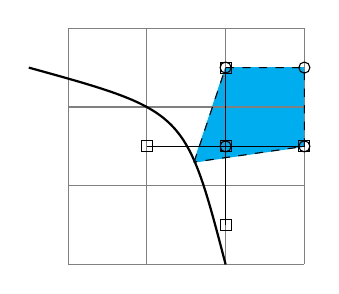
\begin{tikzpicture}
%stencil
%\filldraw[cyan] (0.5,0) rectangle (1.5,1);%shade
\filldraw[cyan] (0.1,-0.2) -- (0.5,1) -- (1.5,1) -- (1.5,0) -- cycle;

%grid
%horizontal
\draw[gray, thin] (-1.5,1.5) -- (1.5,1.5);
\draw[gray, thin] (-1.5,0.5) -- (1.5,0.5);
\draw[gray, thin] (-1.5,-0.5) -- (1.5,-0.5);
\draw[gray, thin] (-1.5,-1.5) -- (1.5,-1.5);
%vertical
\draw[gray, thin] (-1.5,1.5) -- (-1.5,-1.5);
\draw[gray, thin] (-0.5,1.5) -- (-0.5,-1.5);
\draw[gray, thin] (0.5,1.5) -- (0.5,-1.5);
\draw[gray, thin] (1.5,1.5) -- (1.5,-1.5);

%outline
\draw[black, thin, dashed] (0.1,-0.2) -- (0.5,1) -- (1.5,1) -- (1.5,0) -- cycle;
%Interp stencil nodes
\draw [black] (0.5,1) circle (2pt);
\draw [black] (1.5,1) circle (2pt);
\draw [black] (1.5,0) circle (2pt);
\draw [black] (0.5,0) circle (2pt);
%ns stencil nodes
\draw [black] ([xshift=-2pt,yshift=-2pt]0.5,1) rectangle ++(4pt,4pt);
\draw [black] ([xshift=-2pt,yshift=-2pt]1.5,0) rectangle ++(4pt,4pt);
\draw [black] ([xshift=-2pt,yshift=-2pt]0.5,-1) rectangle ++(4pt,4pt);
\draw [black] ([xshift=-2pt,yshift=-2pt]-0.5,0) rectangle ++(4pt,4pt);
\draw [black] ([xshift=-2pt,yshift=-2pt]0.5,0) rectangle ++(4pt,4pt);
%ns stencil lines
\draw [black] (-0.5,0) -- (1.5,0);
\draw [black] (0.5,1) -- (0.5,-1);
%body
\draw[black, thick] (0.5,-1.5) .. controls (-0.01,0.45) .. (-2,1); 

\end{tikzpicture}


\end{document}
